\chapter{\ac{icdo} classification}
\label{ch:icdo}

\section{Dataset}
We collected a set of $1\,592\,385$ anatomopathological exam results
from Tuscany region in the period 2004-2013. About $6\%$
of these records refer to a positive tumor
diagnosis and have topological and morphological ICD-O3 labels,
determined by tumor registry experts. Other reports are associated
with non-cancerous tissues and with unlabeled records. When multiple
pathological records for the
same patient existed for the same tumor, experts selected the most
informative report in order to assign the ICD-O3 code to that tumor
case, leaving a set of $94\,524$ labeled tumor cases.

Histological exam records consist of three free-text fields (not all
of them always filled-in), reporting tissue macroscopy, diagnosis,
and, in some cases, the patient's anamnesis. We found that field
semantics was not always used consistently and that the amount of
provided details varied significantly from extremely synthetic to very
detailed assessments of the morphology and the diagnosis. Field length
ranged from $0$ to $1\,368$ words, with first quartile, median and
third quartile respectively 34, 62, 134. For these reasons we merged
the three text fields
into a single text document, did not apply any conflation (except for
case normalization) kept punctuation. We finally removed duplicate
reports and reports labeled with extremely rare (1048
samples that not
appear in either training, validation, and test sets) ICD-O3 codes. We
obtained in the end 
a dataset suitable for supervised learning consisting of $85\,170$
labeled records over $203$ morphological classes and $68$
topological classes (see below).

\section{Prediction tasks}
A topographical \ac{icdo3} code is structured as \emph{Cmm.s} where
\emph{mm} and \emph{s} represent the main site and the subsite,
respectively. For example, \emph{C50.2}
is the code for the upper-inner quadrant (\emph{2}) of breast (\emph{50}).

A morphological \ac{icdo3} code is structured as \emph{tttt/b}
where \emph{tttt} and \emph{b} represent the cell type and the tumor
behavior (benign, uncertain, in-situ, malignant primary site,
malignant metastatic site), respectively. For example, \emph{8140/3}
is the code for an adenocarcinoma (\emph{adeno 8140};
\emph{carcinoma 3}).

We defined two multi-class classification tasks: (1) main tumor site
prediction ($68$ mutually exclusive classes) and (2) morphology
prediction ($203$ mutually exclusive
classes). Although the two tasks maybe somewhat correlated, we did not
attempt multi-task approaches given the small number of tasks and
large enough size of the dataset.

As shown in \cref{fig:classDist}, the dataset is highly unbalanced.
\begin{figure}
  \centering
  \includegraphics[width=\floatwidth]{img/classDist-icdo3-site.pdf}
  \caption{Documents in classes (ordered by
    frequency).}
  \label{fig:classDist}
\end{figure}

\subsection{Recurrent Neural Networks}
\label{sec:rnn}
In our setting, a dataset $\mathcal{D}=\{(\vect{x}^{(i)},y^{(i)})\}$
consists of variable length sequence vectors $\vect{x}^{(i)}$, where
$x^{(i)}_t$, for $t=1,\dots,T^{(i)}$ is the $t$-th word in the $i$-th
document, and associated target classes
$y^{(i)}\in\{1,\dots,K\}$. Unless necessary, we will drop the
superscript in the following to keep notation simple.  Sequences will
be denoted in boldface. The RNN-based sequence classifiers used in
this work compute their predictions $f(\vect{x})$ as follows:
\begin{align}
  e_t &=& E(\vect{x};\theta^e),\label{eq:embed}\\
  h^f_t &=& F(e_t,h^f_{t-1};\theta^f),\label{eq:maxModelRL}\\  
  h^b_t &=& R(e_t,h^r_{t+1};\theta^r),\label{eq:maxModelRR}\\
  u_t &=& G(h_t;\theta^h),\label{eq:maxModelF}\\
  \phi & =& A(\vect{h},\vect{u};\theta^a),\label{eq:aggregation}\\
  f(\vect{x}) &=& g(\phi;\theta^c).\label{eq:maxModelC}
\end{align}
$E$ is an embedding function mapping words into $p$-dimensional real
vectors (where embedding parameters $\theta_e$ can be either
pretrained and adjustable or fixed, see Section~\ref{sec:word-vectors}
below.  Functions $F$ and $R$ corresponds to (forward and reverse)
dynamics that can be described in term of several (possibly layered)
recurrent cells. In this work we focus on gated recurrent unit (GRU)
cells~\cite{cho2014properties} for their simplicity and because
preliminary experiments revealed no advantages over long-short term
memory cells~\cite{hochreiter1997long} on our data. Each vector $h_t$,
the concatenation of $h^l_t$ and $h^r_t$, can be interpreted as latent
representations of the information contained at position $t$ in the
document. $G$ is an additional layer mapping each latent vector into a
vector $u_t$ that can be seen as contextualized representation of the
word at position $t$. $A$ is an aggregation function that creates a
single $d$-dimensional representation vector for the entire sequence
and $g$ is a softmax layer. Possible choices for the aggregator
function include:
\begin{itemize}
\item $\phi=(h^f_T,h^r_1)$, which just
  extract the extreme latent representations; these may be in
  principle sufficient since they depend on the whole sequence due to
  bidirectional dynamics; note however that this approach may require
  long-term dependencies to be effectively learned.
\item
  $\phi = \sum_t a_t(\vect{u};\theta^a) h_t$,
  using an attention mechanism as in~\cite{yang_hierarchical_2016}; in
  this case, (scalar) attention weights are computed as
  $$
  a_t(\vect{u};\theta^a) = \frac{e^{\langle \theta^a, u_t\rangle}}
  {\sum_s{e^{\langle \theta^a, u_s\rangle}}}
  $$
\item $\phi = \max_t u_t$ where the maximum is taken element-wise
  along the sequence; this approach can be interpreted either as a
  simplified (parameter-less) attention mechanism or a bag-layer as
  proposed in the context of multi-instance
  learning~\cite{tibo2017network}; in this case each ``feature''
  $\phi_j$ will be positive if at least one of $u_{j,1},\dots,u_{j,T}$
  is positive; the resulting classifier will find it easy to create
  decision rules predicting a document as belonging to a certain class
  if a given set of contextualized word representations are present
  and another given set of contextualized word representations are
  absent in the sequence.
\end{itemize}

The parameters $\theta^f,\theta^r,\theta^h$ and $\theta^a$ (if
present) are determined by minimizing a loss function $\loss$
(categorical cross-entropy in our case) on training data:
\begin{equation}
  \hat \theta = \mathrm{arg}\min_\theta\sum_{(\vect{x},y)\in\mathcal{D}}\loss\left(y,f(\vect{x})\right).
\end{equation}


\section{Baseline}

\subsubsection{Linear classifiers}
The classic approach is to employ bag-of-words
representations of textual documents.
%In this approach, a document is 
%described by a \textit{set} or a \textit{multiset} of words.
%Multisets allow one to take into account the number of occurrences of
%a word in the document.
Vector representations of documents are easily
derived from bags-of-words either by using indicator vectors or taking
into account the number of occurrences of each word using the
\ac{tfidf}\cite{manning_introduction_2008}. In those representations,
frequent and non-specific terms receive a lower weight.

Bag-of-words representations (including those employing bigrams or
trigrams) enable the application of very simple text classifiers such
as \ac{nb} or \ac{svm} \cite{cortes-support-1995}, but they
suffer two fundamental problems. First, the relative order of terms in
the documents is lost, making it impossible to take advantage of the
syntactic structure of the sentences. Second, distinct words have an
orthogonal representation even when they are semantically
close. As detailed in the next section, word vectors can be used to
address the second limitation and also allow us to take advantage of
unlabeled data, which can be typically be obtained in large amounts
and with little cost.

\subsubsection{\acs{bert}}
\ac{bert} \cite{devlin2018bert} is a recent model that represents the
state of the art in many \ac{nlp} related tasks
\cite{chatterjee2019semeval,hu2019introductory,lee2019biobert,tshitoyan2019unsupervised}.
It is a
bi-directional pre-training model backboned by the Transformer Encoder
\cite{vaswani2017attention}. It is an attention-based technique that
learns context-dependent word representation on large unlabeled
corpora, and then the model is fine tuned end to end on specific labeled
tasks. During pre-training, the model is trained
on unlabeled data over two different tasks. In \ac{mlm} some tokens
are masked and the model is trained to predict those token based on
the context. In \ac{nsp} the model is trained to understand the
relationship between sentences predicting if two sentences are actually
consecutive or if they where randomly replaced (with 50\%
probability). After the pre-training, the model is fine-tuned to the
specific task.


\subsection{Hyperparameters}
The hyperparameters $\xi=\xi^l\cup\xi^r\cup\xi^h\cup\xi^c$ define the
structure of the model. Regarding $\xi^l=\xi^r$ they define the type
of \ac{rnn} that in our experiments can be \ac{lstm} or \ac{gru}, the
number of stacked \ac{rnn} layers and the dimension of each
layer. $\xi^h$ defines the number of layers in the first
\ac{mlp} and their
dimensions, moreover it defines the type of aggregating function $f$
that in our experiments can be one of
\begin{align}
  f(\vect{a},\vect{b}) &= \left[\max(a_1,b_1),\dots,\max(a_l,b_l)\right];\\
  f(\vect{a},\vect{b}) &= \left[\frac{a_1+b_1}{2},\dots,\frac{a_l+b_l}{2}\right];\\
  f(\vect{a},\vect{b}) &= \left[a_1,\dots,a_l,b_1,\dots,b_l\right].\label{eq:aggregation}
\end{align}
$\xi^c$ defines the number of layers and their dimensions of the
final classifier. The number of layers defined in $\xi^h$ can be
equal to $0$. In such case, $\vect{h}_{i,j}$ is calculated:
\begin{equation*}
  \vect{h}_{i,j} = f(\vect{h}^l_{i,j},\vect{h}^r_{i,j}).
\end{equation*}
Also the number of layers defined in $\xi^c$ can be equal to $0$. In
such case $\vect{\hat{y}}_i$ is calculated:
\begin{equation*}
  \vect{\hat y}_i = \max_j(\vect{h}_{i,j}).
\end{equation*}

\section{Results}
\subsection{Artificial dataset}\label{sec:experiments}
Classic \ac{rnn} approaches exhibit some limits related to
memory. We designed an artificial experiment in
order to investigate how \ac{rnn} and \ac{max} address those
problems. The dataset 
$D=(\vect{X}\in [0,\dots,9]^{n\times m},\vect{y}\in [0,1]^n)$ is
composed of $n$ sequences of length
$m$ of digits $x_{i,j}\in[0,\dots,9]$. If the $i$-th sequence contains
at least three consecutive digits
$x_{i,j-1},x_{i,j},x_{i,j+1}$ that concatenated represents a prime
number then the
sample is positive and labeled with $y_i=1$, otherwise is negative and
$y_i=0$.

We realized a series
$D^{(m)}=(\vect{X}^{(m)},\vect{y}^{(m)})$ of balanced
datasets of increasing complexity. Each $D^{(m)}$ has $100\ 000$
samples with 
sequence lengths of $m\in
[100,200,300,400,500,600,700,800,900,1000]$. We trained two models on
all the datasets: a plain \ac{gru} with hidden dimension $32$ and a
\ac{max} with same hidden dimension $32$. 

\begin{figure}
  \centering
  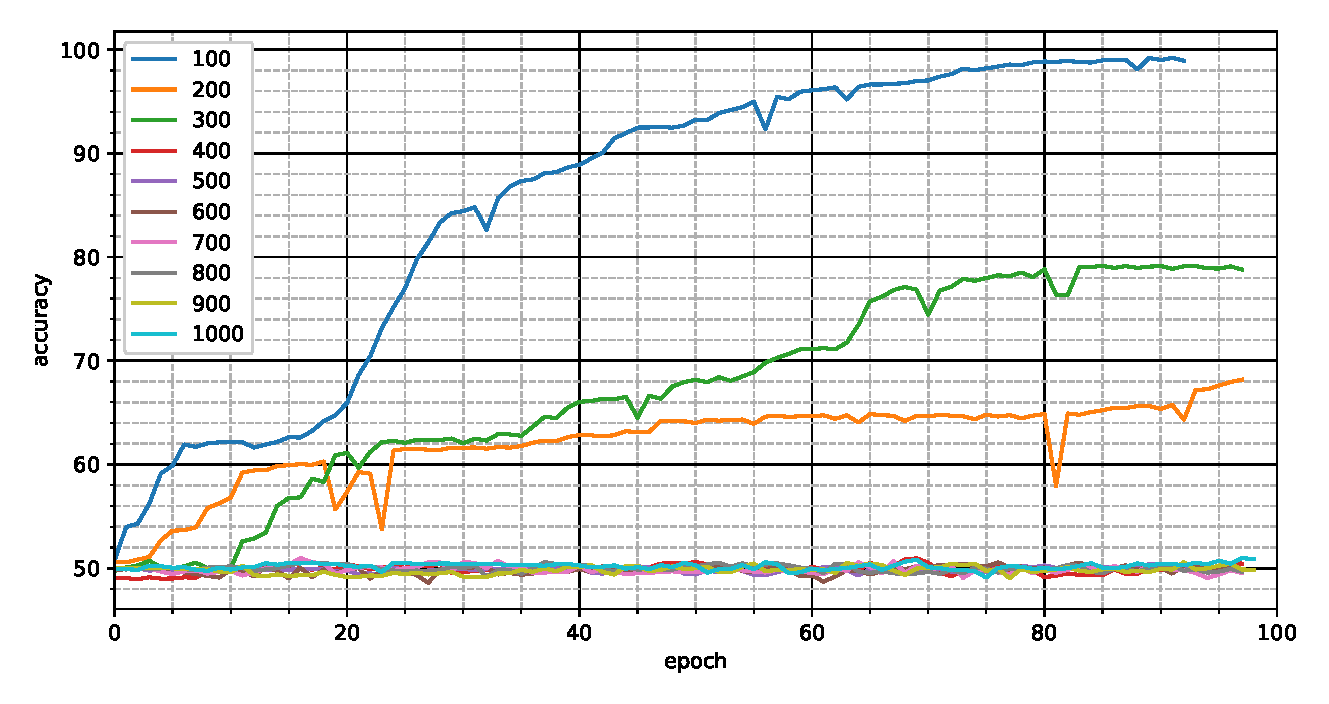
\includegraphics[width=\floatwidth]{imgMax/accuracy-base.eps}
  \caption{Accuracy of plain \ac{gru} on $D^{(m)}$ for different dimensions of $m$.}
  \label{fig:testAccBase}
\end{figure}

\begin{figure}
  \centering
  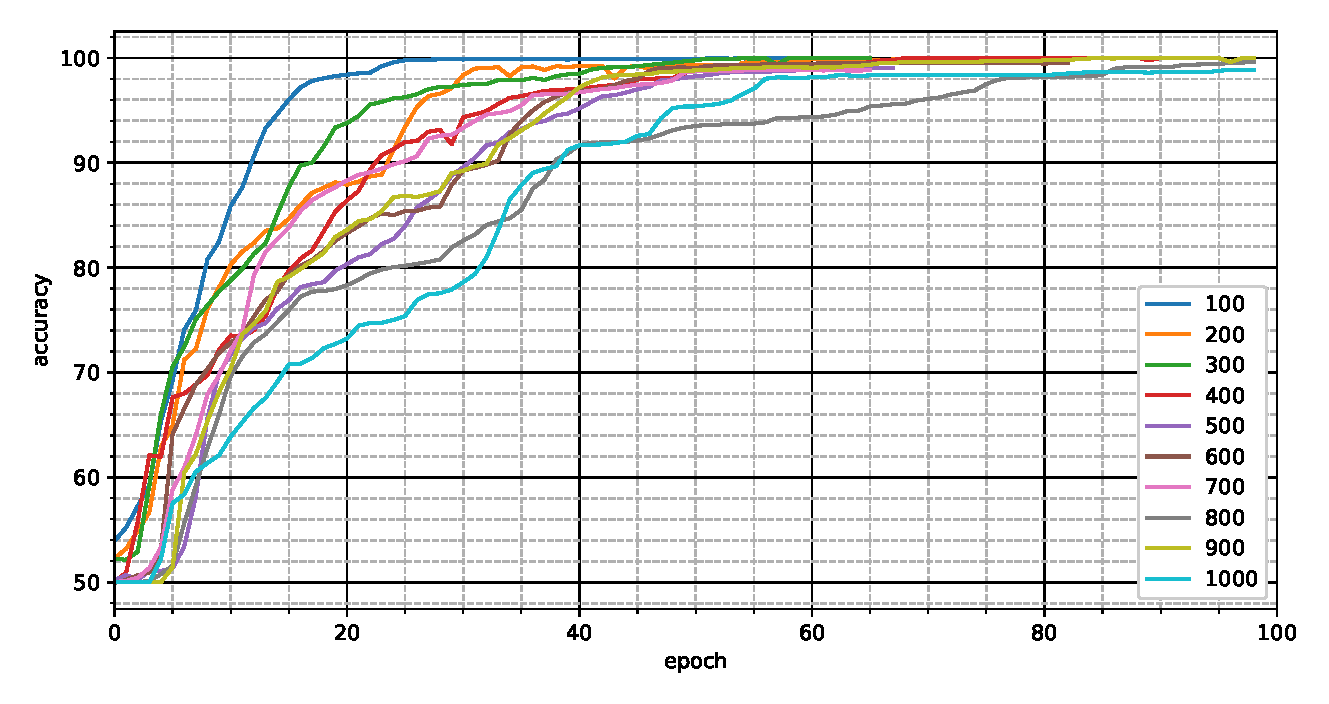
\includegraphics[width=\floatwidth]{imgMax/accuracy-max.eps}
  \caption{Accuracy of \ac{max} on $D^{(m)}$ for different dimensions of $m$.}
  \label{fig:testAccMax}
\end{figure}

In \cref{fig:testAccBase} and \cref{fig:testAccMax} we compare
the learning curves of the base model with \ac{max}. The \ac{gru}
model degrades rapidly respect \ac{max}, under the assumption of
having the same number of parameters.

\subsection{Interpretability}
\ac{max} is flexible enough to gain interpretability under certain
assumptions. Setting in $\xi^c$ in \eqref{eq:maxModelC} the number of
layers to 0 implies that 
the dimension of the last layer in $\xi^h$ in \eqref{eq:maxModelF}
needs to be equal to the
output dimension. We hypothesize that in this setting, the values of
$\vect{h}_{i,j}$ collect information on the importance of the area
around $x_{i,j}$ for the purpose of classification task. This
information can be
used to interpret the model decision. To validate the
hypothesis we performed the same experiment of \cref{sec:experiments}
with an interpretable model with a comparable number of parameters. We
set to 0 the number of layers in \eqref{eq:maxModelC} and to 1 with an
output dimension of 1  in
\eqref{eq:maxModelF}. 

\begin{figure}
  \centering
  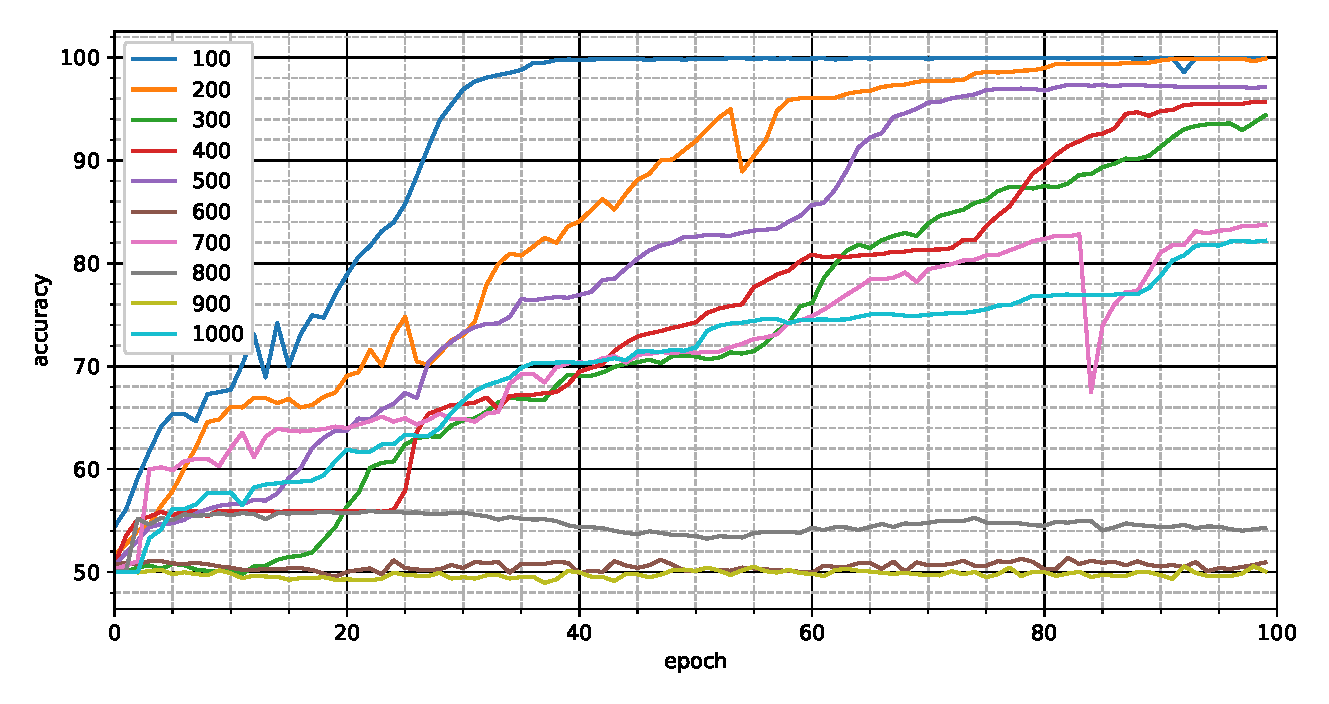
\includegraphics[width=\floatwidth]{imgMax/accuracy-int.eps}
  \caption{Accuracy of interpretable \ac{max} on $D^{(m)}$ for different dimensions of $m$.}
  \label{fig:testAccInt}
\end{figure}
\begin{figure}
  \centering
  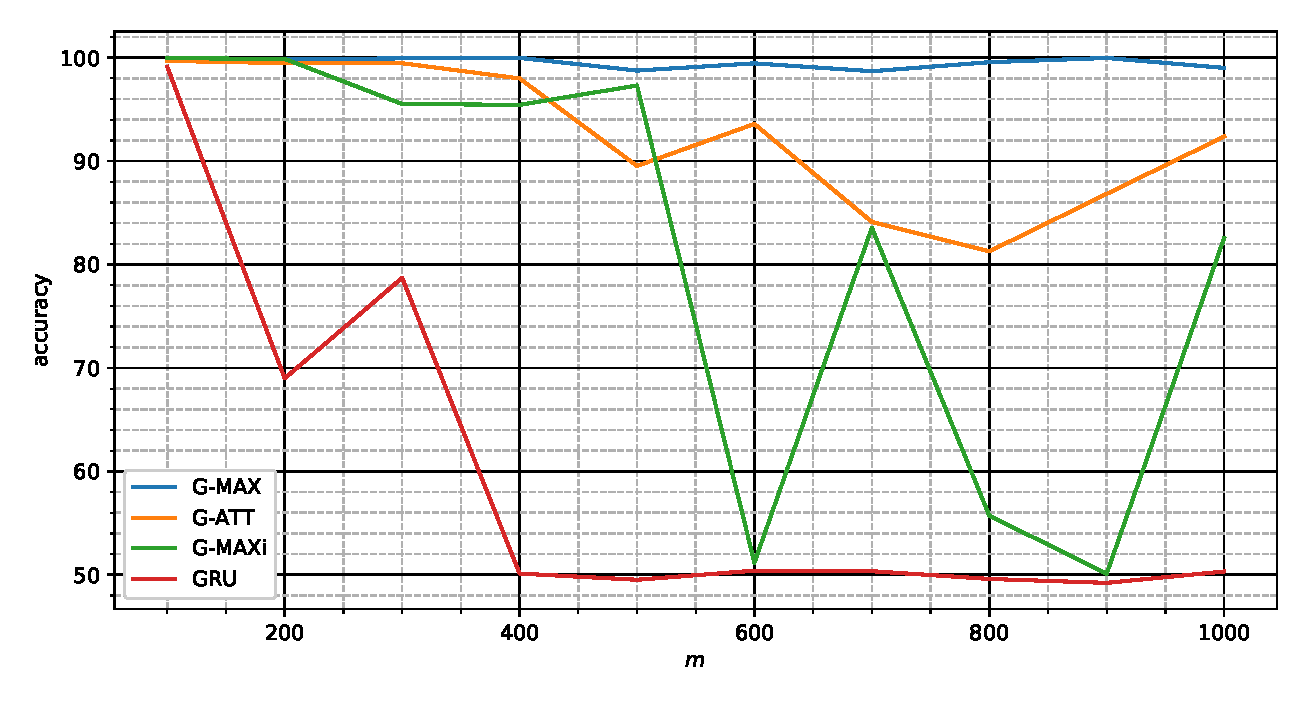
\includegraphics[width=\floatwidth]{imgMax/maxBaseDiff.eps}
  \caption{Max reached accuracy of \ac{max} and \ac{gru} models on $D^{(m)}$ for different dimensions of $m$.}
  \label{fig:testAccDiff}
\end{figure}
\begin{figure}
  \centering
  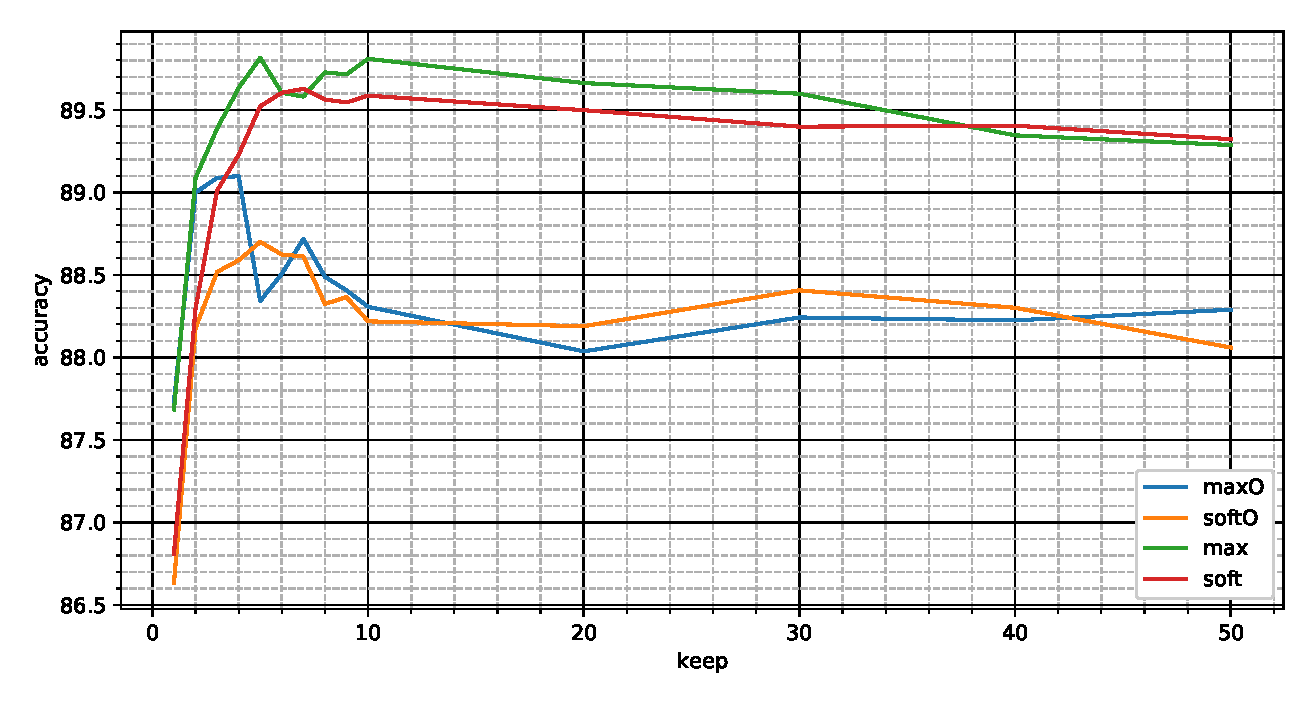
\includegraphics[width=\floatwidth]{img/plotSintex.eps}
  \caption{.}
  \label{fig:sintex}
\end{figure}

\begin{figure}
  \centering
  \footnotesize
  \begin{tabular}{|p{\floatwidth}|}
    \hline
    \attvisB{0}{5}{0} \attvisB{9}{6}{0} \attvisB{2}{7}{0} \attvisB{1}{7}{0} \attvisB{8}{5}{0} \attvisB{4}{5}{0} \attvisB{2}{5}{0} \attvisB{8}{5}{0} \attvisB{9}{6}{0} \attvisB{1}{6}{0} \attvisB{4}{5}{0} \attvisB{6}{5}{0} \attvisB{8}{6}{0} \attvisB{8}{5}{0} \attvisB{6}{4}{0} \attvisB{6}{5}{0} \attvisB{8}{6}{0} \attvisB{7}{7}{0} \attvisB{3}{5}{0} \attvisB{0}{5}{0} \attvisB{2}{5}{0} \attvisB{5}{5}{0} \attvisB{9}{7}{0} \attvisB{7}{7}{0} \attvisB{9}{6}{0} \attvisB{5}{5}{0} \attvisB{8}{5}{0} \attvisB{2}{5}{0} \attvisB{4}{6}{0} \attvisB{9}{6}{0} \attvisB{5}{5}{0} \attvisB{5}{5}{0} \attvisB{6}{5}{0} \attvisB{5}{6}{0} \attvisB{1}{7}{0} \attvisB{7}{7}{0} \attvisB{6}{5}{0} \attvisB{3}{5}{0} \attvisB{2}{6}{0} \attvisB{2}{5}{0} \attvisB{2}{7}{0} \attvisB{1}{6}{100} \attvisB{3}{5}{100} \attvisB{1}{100}{100} \attvisB{2}{5}{0} \attvisB{5}{5}{0} \attvisB{0}{5}{0} \attvisB{8}{5}{0} \attvisB{9}{6}{0} \attvisB{5}{5}{0} \attvisB{4}{6}{0} \attvisB{0}{5}{0} \attvisB{3}{5}{0} \attvisB{2}{5}{0} \attvisB{3}{5}{0} \attvisB{0}{5}{0} \attvisB{6}{4}{0} \attvisB{0}{5}{0} \attvisB{0}{5}{0} \attvisB{8}{5}{0} \attvisB{6}{5}{0} \attvisB{7}{7}{0} \attvisB{9}{7}{0} \attvisB{1}{6}{0} \attvisB{6}{5}{0} \attvisB{4}{6}{0} \attvisB{0}{5}{0} \attvisB{5}{5}{0} \attvisB{7}{7}{0} \attvisB{0}{5}{0} \attvisB{6}{4}{0} \attvisB{4}{6}{0} \attvisB{6}{5}{0} \attvisB{0}{6}{0} \attvisB{6}{5}{0} \attvisB{1}{6}{0} \attvisB{5}{4}{0} \attvisB{4}{6}{0} \attvisB{3}{5}{0} \attvisB{2}{6}{0} \attvisB{5}{5}{0} \attvisB{2}{5}{0} \attvisB{6}{5}{0} \attvisB{7}{7}{0} \attvisB{4}{5}{0} \attvisB{2}{5}{0} \attvisB{5}{5}{0} \attvisB{2}{5}{0} \attvisB{5}{5}{0} \attvisB{8}{5}{0} \attvisB{9}{6}{0} \attvisB{9}{6}{0} \attvisB{5}{6}{0} \attvisB{7}{7}{0} \attvisB{6}{4}{0} \attvisB{5}{5}{0} \attvisB{4}{5}{0} \attvisB{2}{6}{0} \attvisB{7}{7}{0} \attvisB{9}{6}{0}
\\
    \hline
    \attvisB{1}{7}{0} \attvisB{8}{5}{0} \attvisB{4}{6}{0} \attvisB{9}{6}{0} \attvisB{8}{6}{0} \attvisB{0}{6}{0} \attvisB{7}{7}{0} \attvisB{9}{6}{0} \attvisB{2}{5}{0} \attvisB{6}{5}{0} \attvisB{1}{6}{0} \attvisB{0}{5}{0} \attvisB{2}{5}{0} \attvisB{9}{6}{0} \attvisB{2}{5}{0} \attvisB{3}{5}{0} \attvisB{4}{6}{0} \attvisB{8}{5}{0} \attvisB{8}{5}{0} \attvisB{9}{6}{0} \attvisB{3}{5}{0} \attvisB{2}{5}{0} \attvisB{3}{5}{0} \attvisB{8}{6}{0} \attvisB{2}{5}{0} \attvisB{2}{5}{0} \attvisB{4}{6}{0} \attvisB{3}{6}{0} \attvisB{8}{6}{0} \attvisB{7}{7}{0} \attvisB{8}{5}{0} \attvisB{5}{5}{0} \attvisB{0}{5}{0} \attvisB{0}{5}{0} \attvisB{1}{6}{0} \attvisB{0}{5}{0} \attvisB{4}{5}{0} \attvisB{3}{5}{0} \attvisB{8}{6}{0} \attvisB{2}{5}{0} \attvisB{6}{4}{0} \attvisB{5}{5}{0} \attvisB{0}{5}{0} \attvisB{5}{5}{0} \attvisB{3}{5}{0} \attvisB{5}{5}{0} \attvisB{4}{5}{0} \attvisB{2}{5}{0} \attvisB{5}{5}{0} \attvisB{3}{6}{0} \attvisB{0}{5}{0} \attvisB{9}{6}{0} \attvisB{5}{6}{0} \attvisB{7}{7}{0} \attvisB{2}{5}{0} \attvisB{9}{6}{0} \attvisB{0}{6}{0} \attvisB{0}{5}{0} \attvisB{1}{7}{0} \attvisB{7}{7}{0} \attvisB{7}{7}{0} \attvisB{7}{6}{0} \attvisB{9}{6}{0} \attvisB{1}{7}{0} \attvisB{2}{6}{0} \attvisB{6}{5}{0} \attvisB{6}{4}{0} \attvisB{9}{6}{0} \attvisB{8}{6}{0} \attvisB{5}{5}{0} \attvisB{8}{6}{0} \attvisB{1}{7}{0} \attvisB{7}{7}{0} \attvisB{1}{7}{0} \attvisB{6}{4}{0} \attvisB{4}{6}{0} \attvisB{6}{5}{0} \attvisB{5}{6}{0} \attvisB{2}{6}{0} \attvisB{7}{7}{0} \attvisB{0}{6}{0} \attvisB{0}{5}{0} \attvisB{9}{6}{0} \attvisB{6}{4}{0} \attvisB{8}{7}{0} \attvisB{7}{7}{0} \attvisB{6}{5}{0} \attvisB{7}{7}{0} \attvisB{4}{5}{0} \attvisB{2}{5}{0} \attvisB{3}{5}{0} \attvisB{1}{6}{0} \attvisB{8}{5}{0} \attvisB{9}{6}{0} \attvisB{2}{5}{0} \attvisB{6}{5}{0} \attvisB{7}{7}{0} \attvisB{1}{7}{0} \attvisB{4}{6}{0} \attvisB{7}{7}{0}
\\
    \hline
    \attvisB{3}{5}{0} \attvisB{2}{6}{0} \attvisB{8}{5}{0} \attvisB{4}{5}{0} \attvisB{0}{6}{0} \attvisB{7}{6}{0} \attvisB{1}{6}{0} \attvisB{4}{5}{0} \attvisB{8}{5}{0} \attvisB{0}{5}{0} \attvisB{4}{5}{0} \attvisB{2}{5}{0} \attvisB{9}{6}{0} \attvisB{6}{4}{0} \attvisB{3}{6}{0} \attvisB{6}{6}{0} \attvisB{1}{6}{0} \attvisB{5}{4}{0} \attvisB{5}{5}{0} \attvisB{9}{7}{0} \attvisB{7}{7}{0} \attvisB{3}{5}{0} \attvisB{4}{6}{0} \attvisB{0}{5}{0} \attvisB{5}{5}{0} \attvisB{0}{4}{0} \attvisB{2}{5}{0} \attvisB{8}{5}{100} \attvisB{0}{5}{100} \attvisB{9}{6}{100} \attvisB{0}{100}{0} \attvisB{9}{6}{0} \attvisB{3}{5}{0} \attvisB{4}{5}{0} \attvisB{6}{5}{0} \attvisB{5}{5}{0} \attvisB{4}{6}{0} \attvisB{9}{7}{0} \attvisB{6}{5}{0} \attvisB{1}{6}{0} \attvisB{5}{4}{0} \attvisB{5}{5}{0} \attvisB{6}{4}{0} \attvisB{0}{5}{0} \attvisB{3}{5}{0} \attvisB{5}{5}{0} \attvisB{7}{7}{0} \attvisB{5}{4}{0} \attvisB{3}{5}{0} \attvisB{9}{5}{0} \attvisB{4}{6}{0} \attvisB{5}{5}{0} \attvisB{0}{5}{0} \attvisB{1}{7}{0} \attvisB{1}{6}{0} \attvisB{9}{6}{0} \attvisB{5}{6}{0} \attvisB{9}{6}{0} \attvisB{0}{6}{0} \attvisB{0}{6}{0} \attvisB{7}{6}{0} \attvisB{0}{5}{0} \attvisB{3}{5}{0} \attvisB{2}{5}{0} \attvisB{6}{5}{0} \attvisB{7}{7}{0} \attvisB{0}{7}{0} \attvisB{7}{6}{0} \attvisB{4}{6}{0} \attvisB{8}{5}{0} \attvisB{8}{5}{0} \attvisB{0}{5}{0} \attvisB{1}{7}{0} \attvisB{7}{7}{0} \attvisB{6}{5}{0} \attvisB{5}{5}{0} \attvisB{2}{5}{0} \attvisB{2}{5}{0} \attvisB{0}{5}{0} \attvisB{9}{6}{0} \attvisB{4}{6}{0} \attvisB{9}{6}{0} \attvisB{7}{6}{0} \attvisB{4}{6}{0} \attvisB{6}{5}{0} \attvisB{6}{5}{0} \attvisB{5}{6}{0} \attvisB{1}{6}{0} \attvisB{9}{6}{0} \attvisB{6}{4}{0} \attvisB{6}{6}{0} \attvisB{7}{7}{0} \attvisB{2}{6}{0} \attvisB{1}{6}{0} \attvisB{9}{6}{0} \attvisB{8}{7}{0} \attvisB{7}{7}{0} \attvisB{5}{4}{0} \attvisB{6}{4}{0} \attvisB{5}{5}{0}
\\
    \hline
    \attvisB{7}{7}{0} \attvisB{1}{6}{0} \attvisB{0}{5}{0} \attvisB{8}{5}{0} \attvisB{9}{6}{0} \attvisB{9}{6}{0} \attvisB{0}{6}{0} \attvisB{8}{5}{0} \attvisB{3}{5}{0} \attvisB{5}{5}{0} \attvisB{8}{6}{0} \attvisB{1}{6}{0} \attvisB{9}{6}{0} \attvisB{4}{6}{0} \attvisB{9}{6}{0} \attvisB{2}{5}{0} \attvisB{6}{4}{0} \attvisB{0}{6}{0} \attvisB{4}{5}{0} \attvisB{2}{6}{0} \attvisB{7}{7}{0} \attvisB{0}{5}{0} \attvisB{0}{6}{0} \attvisB{6}{5}{0} \attvisB{1}{6}{0} \attvisB{2}{5}{0} \attvisB{0}{6}{0} \attvisB{7}{6}{0} \attvisB{3}{5}{0} \attvisB{5}{5}{0} \attvisB{2}{6}{0} \attvisB{7}{7}{0} \attvisB{4}{5}{0} \attvisB{4}{5}{0} \attvisB{6}{5}{0} \attvisB{2}{5}{0} \attvisB{5}{5}{0} \attvisB{5}{5}{0} \attvisB{8}{5}{0} \attvisB{4}{5}{0} \attvisB{4}{5}{0} \attvisB{8}{5}{0} \attvisB{4}{6}{0} \attvisB{3}{6}{0} \attvisB{7}{7}{0} \attvisB{2}{5}{0} \attvisB{3}{6}{0} \attvisB{5}{5}{0} \attvisB{1}{7}{0} \attvisB{7}{7}{0} \attvisB{1}{7}{0} \attvisB{7}{7}{0} \attvisB{5}{5}{0} \attvisB{5}{5}{0} \attvisB{2}{5}{0} \attvisB{5}{5}{0} \attvisB{4}{7}{0} \attvisB{5}{6}{0} \attvisB{1}{6}{0} \attvisB{6}{5}{0} \attvisB{9}{6}{0} \attvisB{3}{5}{0} \attvisB{4}{6}{0} \attvisB{3}{5}{0} \attvisB{6}{5}{0} \attvisB{0}{6}{0} \attvisB{9}{6}{0} \attvisB{6}{5}{0} \attvisB{1}{7}{0} \attvisB{8}{5}{0} \attvisB{2}{5}{0} \attvisB{0}{6}{0} \attvisB{7}{7}{0} \attvisB{3}{5}{0} \attvisB{1}{6}{0} \attvisB{0}{5}{0} \attvisB{6}{5}{0} \attvisB{1}{7}{0} \attvisB{1}{6}{0} \attvisB{6}{4}{0} \attvisB{8}{5}{0} \attvisB{0}{5}{0} \attvisB{4}{6}{0} \attvisB{3}{6}{0} \attvisB{7}{7}{0} \attvisB{0}{5}{0} \attvisB{6}{4}{0} \attvisB{2}{5}{0} \attvisB{3}{5}{0} \attvisB{2}{6}{0} \attvisB{0}{5}{0} \attvisB{9}{6}{0} \attvisB{0}{6}{0} \attvisB{8}{5}{0} \attvisB{5}{4}{0} \attvisB{5}{5}{0} \attvisB{9}{6}{0} \attvisB{6}{5}{0} \attvisB{9}{6}{0} \attvisB{9}{6}{0}
\\
    \hline
    \attvisB{0}{5}{0} \attvisB{3}{5}{0} \attvisB{3}{5}{100} \attvisB{9}{6}{100} \attvisB{7}{100}{100} \attvisB{3}{5}{0} \attvisB{6}{5}{0} \attvisB{8}{6}{0} \attvisB{6}{5}{0} \attvisB{2}{7}{0} \attvisB{1}{6}{0} \attvisB{5}{5}{0} \attvisB{2}{5}{0} \attvisB{4}{5}{0} \attvisB{3}{5}{0} \attvisB{8}{6}{0} \attvisB{4}{7}{0} \attvisB{7}{6}{0} \attvisB{2}{6}{0} \attvisB{1}{7}{0} \attvisB{7}{7}{0} \attvisB{2}{5}{0} \attvisB{9}{6}{0} \attvisB{2}{5}{0} \attvisB{3}{5}{0} \attvisB{1}{6}{0} \attvisB{6}{5}{0} \attvisB{0}{6}{0} \attvisB{0}{6}{0} \attvisB{7}{6}{0} \attvisB{2}{6}{0} \attvisB{0}{5}{0} \attvisB{1}{6}{0} \attvisB{4}{5}{0} \attvisB{3}{5}{0} \attvisB{2}{6}{0} \attvisB{0}{5}{0} \attvisB{9}{6}{0} \attvisB{4}{6}{0} \attvisB{3}{5}{0} \attvisB{6}{4}{0} \attvisB{8}{5}{0} \attvisB{8}{5}{0} \attvisB{0}{6}{0} \attvisB{6}{5}{0} \attvisB{1}{6}{0} \attvisB{2}{5}{0} \attvisB{2}{5}{0} \attvisB{6}{5}{0} \attvisB{7}{7}{0} \attvisB{2}{5}{0} \attvisB{6}{4}{0} \attvisB{5}{5}{0} \attvisB{6}{4}{0} \attvisB{6}{5}{0} \attvisB{4}{6}{0} \attvisB{5}{5}{0} \attvisB{5}{5}{0} \attvisB{2}{5}{0} \attvisB{2}{5}{0} \attvisB{2}{6}{0} \attvisB{1}{6}{0} \attvisB{2}{5}{0} \attvisB{3}{6}{0} \attvisB{7}{7}{0} \attvisB{1}{7}{0} \attvisB{8}{5}{0} \attvisB{8}{5}{0} \attvisB{8}{5}{0} \attvisB{2}{5}{0} \attvisB{8}{5}{0} \attvisB{5}{4}{0} \attvisB{8}{5}{0} \attvisB{3}{5}{0} \attvisB{4}{6}{0} \attvisB{8}{5}{0} \attvisB{5}{5}{0} \attvisB{6}{4}{0} \attvisB{8}{6}{0} \attvisB{0}{5}{0} \attvisB{3}{5}{0} \attvisB{6}{4}{0} \attvisB{9}{6}{0} \attvisB{0}{6}{0} \attvisB{6}{4}{0} \attvisB{0}{5}{0} \attvisB{4}{5}{0} \attvisB{0}{5}{0} \attvisB{8}{5}{0} \attvisB{2}{5}{0} \attvisB{4}{6}{0} \attvisB{5}{5}{0} \attvisB{5}{5}{0} \attvisB{2}{5}{0} \attvisB{4}{5}{0} \attvisB{0}{5}{0} \attvisB{8}{5}{0} \attvisB{3}{5}{0} \attvisB{0}{5}{0} \attvisB{8}{5}{0}
\\
    \hline
    \attvisB{1}{7}{0} \attvisB{5}{5}{0} \attvisB{5}{5}{0} \attvisB{8}{5}{0} \attvisB{8}{5}{0} \attvisB{9}{6}{0} \attvisB{8}{6}{0} \attvisB{8}{5}{0} \attvisB{0}{5}{0} \attvisB{3}{5}{0} \attvisB{5}{5}{0} \attvisB{2}{5}{0} \attvisB{0}{5}{0} \attvisB{0}{5}{0} \attvisB{2}{6}{0} \attvisB{7}{7}{0} \attvisB{5}{4}{0} \attvisB{4}{6}{0} \attvisB{2}{5}{0} \attvisB{4}{7}{0} \attvisB{7}{7}{0} \attvisB{0}{5}{0} \attvisB{4}{5}{0} \attvisB{6}{5}{0} \attvisB{5}{5}{0} \attvisB{0}{5}{0} \attvisB{4}{5}{0} \attvisB{0}{5}{0} \attvisB{2}{5}{0} \attvisB{6}{5}{0} \attvisB{7}{7}{0} \attvisB{9}{6}{0} \attvisB{6}{5}{0} \attvisB{9}{6}{0} \attvisB{2}{5}{0} \attvisB{4}{6}{0} \attvisB{7}{7}{0} \attvisB{5}{4}{0} \attvisB{8}{5}{0} \attvisB{4}{7}{0} \attvisB{1}{6}{0} \attvisB{6}{4}{0} \attvisB{5}{6}{0} \attvisB{5}{5}{0} \attvisB{1}{7}{0} \attvisB{1}{6}{0} \attvisB{9}{6}{0} \attvisB{8}{6}{0} \attvisB{2}{5}{0} \attvisB{6}{4}{0} \attvisB{2}{5}{0} \attvisB{6}{4}{0} \attvisB{8}{6}{0} \attvisB{5}{5}{0} \attvisB{4}{6}{0} \attvisB{0}{5}{0} \attvisB{5}{4}{0} \attvisB{5}{5}{0} \attvisB{9}{6}{0} \attvisB{2}{6}{0} \attvisB{5}{5}{0} \attvisB{6}{4}{0} \attvisB{2}{5}{0} \attvisB{9}{6}{0} \attvisB{0}{6}{0} \attvisB{3}{5}{0} \attvisB{8}{6}{0} \attvisB{4}{5}{0} \attvisB{3}{6}{0} \attvisB{7}{7}{0} \attvisB{8}{5}{0} \attvisB{9}{6}{0} \attvisB{1}{7}{0} \attvisB{8}{5}{0} \attvisB{3}{6}{0} \attvisB{7}{7}{0} \attvisB{8}{5}{0} \attvisB{9}{6}{0} \attvisB{8}{6}{0} \attvisB{1}{6}{0} \attvisB{9}{6}{0} \attvisB{6}{4}{0} \attvisB{6}{4}{0} \attvisB{6}{5}{0} \attvisB{7}{7}{0} \attvisB{4}{6}{0} \attvisB{9}{6}{0} \attvisB{4}{6}{0} \attvisB{4}{7}{0} \attvisB{7}{7}{0} \attvisB{8}{5}{0} \attvisB{0}{5}{0} \attvisB{1}{6}{0} \attvisB{8}{5}{0} \attvisB{3}{6}{0} \attvisB{7}{7}{0} \attvisB{8}{5}{0} \attvisB{4}{5}{0} \attvisB{6}{5}{0} \attvisB{6}{5}{0}
\\
    \hline
  \end{tabular}
  \caption{Visualization of outputs prior to the max pooling for some
    samples. Red boxes represent the prime numbers ground
    truth, green highlighting represents the values of $h_{i,j}$ in
    \eqref{eq:maxModelF}.}
  \label{fig:testAttention}
\end{figure}

\begin{figure}
  \centering
  \footnotesize
  \begin{tabular}{|p{\floatwidth}|}
    \hline
    \attvisB{3}{0}{0} \attvisB{6}{0}{0} \attvisB{2}{0}{0} \attvisB{9}{0}{0} \attvisB{4}{0}{0} \attvisB{8}{0}{0} \attvisB{0}{0}{0} \attvisB{6}{0}{0} \attvisB{3}{0}{0} \attvisB{0}{0}{0} \attvisB{4}{0}{0} \attvisB{7}{0}{0} \attvisB{6}{0}{0} \attvisB{5}{0}{0} \attvisB{6}{0}{0} \attvisB{7}{0}{0} \attvisB{5}{0}{0} \attvisB{9}{0}{0} \attvisB{8}{0}{0} \attvisB{6}{0}{0} \attvisB{5}{0}{0} \attvisB{1}{0}{0} \attvisB{2}{0}{0} \attvisB{6}{0}{0} \attvisB{7}{0}{0} \attvisB{8}{0}{0} \attvisB{8}{0}{0} \attvisB{2}{0}{0} \attvisB{2}{0}{0} \attvisB{5}{0}{0} \attvisB{3}{0}{0} \attvisB{1}{0}{0} \attvisB{6}{0}{0} \attvisB{4}{0}{0} \attvisB{4}{0}{0} \attvisB{0}{0}{0} \attvisB{7}{0}{0} \attvisB{4}{0}{0} \attvisB{8}{0}{100} \attvisB{6}{78}{100} \attvisB{3}{0}{100} \attvisB{2}{0}{0} \attvisB{0}{20}{0} \attvisB{6}{0}{0} \attvisB{0}{0}{0} \attvisB{6}{0}{0} \attvisB{2}{0}{0} \attvisB{1}{0}{0} \attvisB{5}{0}{0} \attvisB{5}{0}{0} \attvisB{8}{0}{0} \attvisB{2}{0}{0} \attvisB{4}{0}{0} \attvisB{8}{0}{0} \attvisB{9}{0}{0} \attvisB{0}{0}{0} \attvisB{1}{0}{0} \attvisB{1}{0}{0} \attvisB{2}{0}{0} \attvisB{3}{0}{0} \attvisB{2}{0}{0} \attvisB{7}{0}{0} \attvisB{5}{0}{0} \attvisB{0}{0}{0} \attvisB{1}{0}{0} \attvisB{8}{0}{0} \attvisB{5}{0}{0} \attvisB{2}{0}{0} \attvisB{4}{0}{0} \attvisB{4}{0}{0} \attvisB{7}{0}{0} \attvisB{5}{0}{0} \attvisB{3}{0}{0} \attvisB{6}{0}{0} \attvisB{4}{0}{0} \attvisB{9}{0}{0} \attvisB{0}{0}{0} \attvisB{6}{0}{0} \attvisB{6}{0}{0} \attvisB{2}{0}{0} \attvisB{5}{0}{0} \attvisB{5}{0}{0} \attvisB{5}{0}{0} \attvisB{1}{0}{0} \attvisB{6}{0}{0} \attvisB{1}{0}{0} \attvisB{0}{0}{0} \attvisB{0}{0}{0} \attvisB{6}{0}{0} \attvisB{7}{0}{0} \attvisB{5}{0}{0} \attvisB{9}{0}{0} \attvisB{7}{0}{0} \attvisB{4}{0}{0} \attvisB{4}{0}{0} \attvisB{5}{0}{0} \attvisB{2}{0}{0} \attvisB{4}{0}{0} \attvisB{9}{0}{0} \attvisB{2}{0}{0}

\\
    \hline
    \attvisB{5}{0}{0} \attvisB{3}{0}{0} \attvisB{6}{0}{0} \attvisB{9}{0}{0} \attvisB{0}{0}{0} \attvisB{9}{0}{0} \attvisB{1}{0}{0} \attvisB{8}{0}{0} \attvisB{0}{0}{0} \attvisB{1}{0}{0} \attvisB{5}{0}{0} \attvisB{4}{0}{0} \attvisB{5}{0}{0} \attvisB{0}{0}{0} \attvisB{4}{0}{0} \attvisB{7}{0}{0} \attvisB{1}{0}{0} \attvisB{6}{0}{0} \attvisB{2}{0}{0} \attvisB{3}{0}{0} \attvisB{2}{0}{0} \attvisB{9}{0}{0} \attvisB{2}{0}{0} \attvisB{6}{0}{0} \attvisB{8}{0}{0} \attvisB{8}{0}{0} \attvisB{2}{0}{0} \attvisB{6}{0}{0} \attvisB{1}{0}{0} \attvisB{1}{0}{0} \attvisB{2}{0}{0} \attvisB{3}{0}{0} \attvisB{6}{0}{0} \attvisB{3}{0}{0} \attvisB{6}{0}{0} \attvisB{4}{0}{0} \attvisB{4}{0}{0} \attvisB{6}{0}{0} \attvisB{6}{0}{0} \attvisB{8}{0}{0} \attvisB{9}{0}{0} \attvisB{9}{0}{0} \attvisB{3}{0}{0} \attvisB{5}{0}{0} \attvisB{6}{0}{0} \attvisB{4}{0}{0} \attvisB{2}{0}{0} \attvisB{4}{0}{0} \attvisB{7}{0}{0} \attvisB{0}{0}{0} \attvisB{3}{0}{0} \attvisB{3}{0}{0} \attvisB{8}{0}{0} \attvisB{5}{0}{0} \attvisB{5}{0}{0} \attvisB{4}{0}{0} \attvisB{6}{0}{0} \attvisB{9}{0}{0} \attvisB{2}{0}{0} \attvisB{3}{0}{0} \attvisB{2}{0}{0} \attvisB{9}{0}{0} \attvisB{5}{0}{0} \attvisB{5}{0}{0} \attvisB{3}{0}{0} \attvisB{5}{0}{0} \attvisB{7}{0}{0} \attvisB{8}{0}{0} \attvisB{0}{0}{0} \attvisB{4}{0}{0} \attvisB{7}{0}{0} \attvisB{1}{0}{0} \attvisB{3}{0}{0} \attvisB{6}{0}{0} \attvisB{6}{0}{0} \attvisB{3}{0}{0} \attvisB{8}{0}{0} \attvisB{8}{0}{0} \attvisB{8}{0}{0} \attvisB{8}{0}{0} \attvisB{6}{0}{0} \attvisB{9}{0}{0} \attvisB{6}{0}{0} \attvisB{0}{0}{0} \attvisB{6}{0}{0} \attvisB{4}{0}{100} \attvisB{0}{0}{100} \attvisB{1}{0}{100} \attvisB{5}{8}{0} \attvisB{4}{8}{0} \attvisB{9}{8}{0} \attvisB{5}{8}{0} \attvisB{5}{8}{0} \attvisB{5}{8}{0} \attvisB{9}{8}{0} \attvisB{7}{8}{0} \attvisB{6}{8}{0} \attvisB{5}{8}{0} \attvisB{8}{8}{0} \attvisB{4}{8}{0}

\\
    \hline
    \attvisB{3}{0}{0} \attvisB{2}{0}{0} \attvisB{8}{0}{0} \attvisB{4}{0}{0} \attvisB{0}{0}{0} \attvisB{7}{0}{0} \attvisB{1}{0}{0} \attvisB{4}{0}{0} \attvisB{8}{0}{0} \attvisB{0}{0}{0} \attvisB{4}{0}{0} \attvisB{2}{0}{0} \attvisB{9}{0}{0} \attvisB{6}{0}{0} \attvisB{3}{0}{0} \attvisB{6}{0}{0} \attvisB{1}{0}{0} \attvisB{5}{0}{0} \attvisB{5}{0}{0} \attvisB{9}{0}{0} \attvisB{7}{0}{0} \attvisB{3}{0}{0} \attvisB{4}{0}{0} \attvisB{0}{0}{0} \attvisB{5}{0}{0} \attvisB{0}{0}{0} \attvisB{2}{0}{0} \attvisB{8}{0}{100} \attvisB{0}{0}{100} \attvisB{9}{0}{100} \attvisB{0}{1}{0} \attvisB{9}{1}{0} \attvisB{3}{1}{0} \attvisB{4}{1}{0} \attvisB{6}{1}{0} \attvisB{5}{1}{0} \attvisB{4}{1}{0} \attvisB{9}{1}{0} \attvisB{6}{1}{0} \attvisB{1}{1}{0} \attvisB{5}{1}{0} \attvisB{5}{1}{0} \attvisB{6}{1}{0} \attvisB{0}{1}{0} \attvisB{3}{1}{0} \attvisB{5}{1}{0} \attvisB{7}{1}{0} \attvisB{5}{1}{0} \attvisB{3}{1}{0} \attvisB{9}{1}{0} \attvisB{4}{1}{0} \attvisB{5}{1}{0} \attvisB{0}{1}{0} \attvisB{1}{1}{0} \attvisB{1}{1}{0} \attvisB{9}{1}{0} \attvisB{5}{1}{0} \attvisB{9}{1}{0} \attvisB{0}{1}{0} \attvisB{0}{1}{0} \attvisB{7}{1}{0} \attvisB{0}{1}{0} \attvisB{3}{1}{0} \attvisB{2}{1}{0} \attvisB{6}{1}{0} \attvisB{7}{1}{0} \attvisB{0}{1}{0} \attvisB{7}{1}{0} \attvisB{4}{1}{0} \attvisB{8}{1}{0} \attvisB{8}{1}{0} \attvisB{0}{1}{0} \attvisB{1}{1}{0} \attvisB{7}{1}{0} \attvisB{6}{1}{0} \attvisB{5}{1}{0} \attvisB{2}{1}{0} \attvisB{2}{1}{0} \attvisB{0}{1}{0} \attvisB{9}{1}{0} \attvisB{4}{1}{0} \attvisB{9}{1}{0} \attvisB{7}{1}{0} \attvisB{4}{1}{0} \attvisB{6}{1}{0} \attvisB{6}{1}{0} \attvisB{5}{1}{0} \attvisB{1}{1}{0} \attvisB{9}{1}{0} \attvisB{6}{1}{0} \attvisB{6}{1}{0} \attvisB{7}{1}{0} \attvisB{2}{1}{0} \attvisB{1}{1}{0} \attvisB{9}{1}{0} \attvisB{8}{1}{0} \attvisB{7}{1}{0} \attvisB{5}{1}{0} \attvisB{6}{1}{0} \attvisB{5}{1}{0}

\\
    \hline
  \end{tabular}
  \caption{Visualization of weighted features after softmax for some
    positive samples. Red boxes represent the prime numbers ground
    truth, green highlighting represents the values of $h_{i,j}$ in
    \eqref{eq:softModelF}.}
  \label{fig:testAttentionSoft}
\end{figure}

The degradation of the model in fig. \ref{fig:testAccInt} is worst
compared with the full \ac{max} model in fig. \ref{fig:testAccMax},
but is still better compared with the baseline in
fig. \ref{fig:testAccBase}. Conversely the interpretable model gain
some insights on the decisions. As visible in
fig. \ref{fig:testAttention}, the model performs the classification
task focusing on 
the part of the sequences where the prime numbers are present.

\subsection{Cancer register data}
Machine learning models need a training dataset in order to learn how
to perform predictions. A second test dataset — sampled from the same
distribution — is needed to assess the performances of the
classifier, and a third evaluation dataset is used to tune the
hyperparameters and to stop the training before the model overfits to
the training dataset. We decided to arrange our experiments on cancer
data in 
a setting that simulate a predictive task. We sorted the medical
records by insertion date, then we used the most recent $80\%$ of
records as test 
dataset, an equal amount of the remaining most recent records as
validation dataset, and the rest as training dataset. At the end the
training, validation, and test datasets have respectively $51\,101$,
$17\,034$, and $17\,035$ records.

We used the text in the $1.5$ millions unlabeled records, plus the
text in training datasets to train \ac{glove} word
vectors representations. We trained two different \ac{max} models, one
in an interpretable configuration that we call \maxi{} and one not
interpretable with 
best configuration that we call \maxb{}. We found the hyperparameters
configuration with grid search. 
\maxi{} have one \ac{gru} layer of dimension $256$
for \eqref{eq:maxModelRL} and \eqref{eq:maxModelRR}, 1 layer of
output dimension $68$ with aggregating function \eqref{eq:aggregation}
for \eqref{eq:maxModelF}, and zero layers for \eqref{eq:maxModelC}. 
\maxb{} have
one \ac{gru} layer with
dimension $128$ for \eqref{eq:maxModelRL} and \eqref{eq:maxModelRR},
one \ac{mlp} layer of dimension $512$ with aggregating function
\eqref{eq:aggregation} for \eqref{eq:maxModelF}, and
one layer of output dimension $68$ for \eqref{eq:maxModelC}.

We trained the models minimizing categorical cross entropy with Adam
\cite{kingma2014adam} using a learning rate of $0.001$. The
experiments were performed in \emph{PyTorch} on machines with
\emph{GeForce RTX 2080 Ti} 
GPU using batches of $32$ samples.

We compared \maxb{} and \maxi{} with a baseline of two stacked
bidirectional 
\ac{gru} layer of dimension $256$ and with \ac{bert} pretrained on the
same data where \ac{glove} where trained for the other models, and
fine-tuned on the training set.

\begin{table}
  \centering
  \caption{Results on cancer data}
  \label{tab:results}
  \begin{tabular}{|c|c|c|c|c|c|c|}
    \hline
    &baseline&\ac{bert}&\maxi{}&\softmax{}&\maxb{}\\
    \hline
    \hline
    \textbf{Site}&&&&&\\
    Acc.&0.8977&0.8980&0.8792&0.9008&\textbf{0.9024}\\
    Acc. top3&0.9636&0.9623&0.9533&0.9607&\textbf{0.9658}\\
    Acc. top5&0.9764&0.9768&0.9610&0.9749&\textbf{0.9797}\\
    MAP &0.9331&0.9330&0.9190&0.9341&\textbf{0.9369}\\
    K&0.8848&0.8852&0.8637&0.8883&\textbf{0.8901}\\
    \hline
    \hline
    \textbf{Morpho.}&&&&&\\
    Acc.&0.8266&0.8367&0.7317&\textbf{0.8424}&0.8394 \\
    Acc. top3&0.9402&0.9267&0.9012&0.9445&\textbf{0.9452} \\
    Acc. top5&0.9602&0.9439&0.9305&0.9632&\textbf{0.9634} \\
    MAP&0.8881&0.8870&0.8169&\textbf{0.8973}&0.8962 \\
    K&0.8064&0.8178&0.6964&\textbf{0.8240}&0.8207 \\
    \hline
  \end{tabular}
\end{table}
In \cref{tab:results} we resumed the results of the models on the test
dataset. We report accuracy, \ac{map} and Cohen's kappa score (K).
\ac{map} is used in information
retrieval \cite{manning_introduction_2008}. It expresses how well the
correct class of a sample can be retrieved in 
the first results of the classifier output.
Cohen's kappa score is usually used to assess
the agreement of two annotators \cite{cohen_coefficient_1960}. It
measures the difference between the observed agreement and the
agreement that can happen choosing randomly the class. Can be used to
mitigate the bias caused by the unbalanced data set.

\begin{table}
  \centering
  \ttfamily
  \scriptsize
  \caption{Visualization of interpretable outputs.}
  \label{tab:multiAttention1}
  \begin{tabular}{|c|c|c|}
    \hline
    $y_i$&\textrm{Relevant} $\vect{h}_{i,j}$&$x_{i,j}$\textrm{, relevant} $\vect{h}_{i,j}$\\
    \hline
    61&\begin{minipage}{\attTableIcdoWidth}\att{61}{red}{100} \att{(PROSTATE}{red}{100} \att{GLAND)}{red}{100} \end{minipage}&\begin{minipage}{\attTableTextWidth}\att{DISOMOGENICITA}{red}{0} \att{'}{red}{0} \att{DIFFUSE}{red}{0} \att{.}{red}{0} \att{PSA}{red}{85} \att{NON}{red}{0} \att{PERVENUTO}{red}{0} \att{.}{red}{0} \att{ADENOCARCINOMA}{red}{0} \att{PROSTATICO}{red}{100} \att{A}{red}{0} \att{GRADO}{red}{1} \att{DI}{red}{0} \att{DIFFERENZIAZIONE}{red}{0} \att{MEDIO}{red}{0} \att{-}{red}{0} \att{BASSO}{red}{0} \att{(}{red}{0} \att{GLEASON}{red}{100} \att{3}{red}{4} \att{+}{red}{0} \att{4}{red}{0} \att{)}{red}{0} \att{NEI}{red}{0} \att{PRELIEVI}{red}{0} \att{DI}{red}{0} \att{CUI}{red}{0} \att{AI}{red}{0} \att{NN}{red}{0} \att{.}{red}{0} \att{2}{red}{0} \att{E}{red}{0} \att{3}{red}{0} \att{.}{red}{0} \att{AGOBIOPSIA}{red}{0} \att{DELLA}{red}{0} \att{PROSTATA}{red}{100} \att{:}{red}{0} \att{1}{red}{0} \att{)}{red}{0} \att{1}{red}{0} \att{PRELIEVO}{red}{0} \att{LL}{red}{0} \att{DX}{red}{0} \att{.}{red}{0} \att{2}{red}{0} \att{)}{red}{0} \att{2}{red}{0} \att{PRELIEVI}{red}{0} \att{ML}{red}{0} \att{DX}{red}{0} \att{.}{red}{0} \att{3}{red}{0} \att{)}{red}{0} \att{2}{red}{0} \att{PRELIEVI}{red}{0} \att{M}{red}{0} \att{DX}{red}{0} \att{.}{red}{0} \att{4}{red}{0} \att{)}{red}{0} \att{1}{red}{0} \att{PRELIEVO}{red}{0} \att{M}{red}{0} \att{SX}{red}{0} \att{.}{red}{0} \att{5}{red}{0} \att{)}{red}{0} \att{2}{red}{0} \att{PRELIEVI}{red}{0} \att{ML}{red}{0} \att{SX}{red}{0} \att{.}{red}{0} \att{6}{red}{0} \att{)}{red}{0} \att{1}{red}{0} \att{PRELIEVO}{red}{0} \att{LL}{red}{0} \att{SX}{red}{0} \att{.}{red}{0} \att{7}{red}{0} \att{)}{red}{0} \att{1}{red}{0} \att{PRELIEVO}{red}{0} \att{TRANSIZIONALE}{red}{54} \att{SX}{red}{1} \att{.}{red}{0} \att{8}{red}{0} \att{)}{red}{0} \att{1}{red}{0} \att{PRELIEVO}{red}{0} \att{TRANSIZIONALE}{red}{19} \att{DX}{red}{7} \att{.}{red}{0} \end{minipage}\\ % doc valid 49


    \hline
    20&\begin{minipage}{\attTableIcdoWidth}\att{\att{\att{18}{red}{100}}{green}{0}}{blue}{0} \att{\att{\att{(COLON)}{red}{100}}{green}{0}}{blue}{0} \\\\\att{\att{\att{20}{red}{0}}{green}{100}}{blue}{0} \att{\att{\att{(RECTUM)}{red}{0}}{green}{100}}{blue}{0} \\\\\att{\att{\att{21}{red}{0}}{green}{0}}{blue}{100} \att{\att{\att{(ANUS}{red}{0}}{green}{0}}{blue}{100} \att{\att{\att{AND}{red}{0}}{green}{0}}{blue}{100} \att{\att{\att{ANAL}{red}{0}}{green}{0}}{blue}{100} \att{\att{\att{CANAL)}{red}{0}}{green}{0}}{blue}{100} \end{minipage}&\begin{minipage}{\attTableTextWidth}\att{\att{\att{ISOLATI}{red}{0}}{green}{0}}{blue}{0} \att{\att{\att{FRAMMENTI}{red}{0}}{green}{0}}{blue}{0} \att{\att{\att{RIFERIBILI}{red}{0}}{green}{0}}{blue}{0} \att{\att{\att{AD}{red}{0}}{green}{0}}{blue}{0} \att{\att{\att{ADENOMA}{red}{0}}{green}{0}}{blue}{0} \att{\att{\att{TUBULARE}{red}{100}}{green}{0}}{blue}{0} \att{\att{\att{INTESTINALE}{red}{100}}{green}{1}}{blue}{0} \att{\att{\att{DI}{red}{2}}{green}{0}}{blue}{0} \att{\att{\att{ALTO}{red}{4}}{green}{0}}{blue}{0} \att{\att{\att{GRADO}{red}{1}}{green}{0}}{blue}{0} \att{\att{\att{.}{red}{0}}{green}{0}}{blue}{0} \att{\att{\att{FRAMMENTI}{red}{0}}{green}{0}}{blue}{0} \att{\att{\att{(}{red}{0}}{green}{0}}{blue}{0} \att{\att{\att{NR}{red}{0}}{green}{0}}{blue}{0} \att{\att{\att{.}{red}{0}}{green}{0}}{blue}{0} \att{\att{\att{2}{red}{0}}{green}{0}}{blue}{0} \att{\att{\att{)}{red}{0}}{green}{0}}{blue}{0} \att{\att{\att{DI}{red}{0}}{green}{0}}{blue}{0} \att{\att{\att{POLIPO}{red}{88}}{green}{63}}{blue}{0} \att{\att{\att{PEDUNCOLATO}{red}{100}}{green}{0}}{blue}{0} \att{\att{\att{A}{red}{0}}{green}{0}}{blue}{0} \att{\att{\att{20}{red}{0}}{green}{0}}{blue}{0} \att{\att{\att{CM}{red}{0}}{green}{0}}{blue}{0} \att{\att{\att{DALL}{red}{61}}{green}{0}}{blue}{0} \att{\att{\att{'}{red}{0}}{green}{0}}{blue}{0} \att{\att{\att{ORIFIZIO}{red}{0}}{green}{96}}{blue}{89} \att{\att{\att{ANALE}{red}{0}}{green}{100}}{blue}{100} \att{\att{\att{.}{red}{0}}{green}{30}}{blue}{0} \att{\att{\att{(}{red}{0}}{green}{0}}{blue}{0} \att{\att{\att{ESEGUITA}{red}{0}}{green}{0}}{blue}{0} \att{\att{\att{COLORAZIONE}{red}{0}}{green}{0}}{blue}{0} \att{\att{\att{EMATOSSILINA}{red}{0}}{green}{0}}{blue}{0} \att{\att{\att{-}{red}{0}}{green}{0}}{blue}{0} \att{\att{\att{EOSINA}{red}{0}}{green}{0}}{blue}{0} \att{\att{\att{)}{red}{0}}{green}{0}}{blue}{0} \att{\att{\att{.}{red}{0}}{green}{0}}{blue}{0} \end{minipage}\\ % doc valid 2


    \hline
    %61&\begin{minipage}{\attTableIcdoWidth}\att{61}{red}{100} \att{(PROSTATE}{red}{100} \att{GLAND)}{red}{100} \end{minipage}&\begin{minipage}{\attTableTextWidth}\att{DISOMOGENICITA}{red}{0} \att{'}{red}{0} \att{DIFFUSE}{red}{0} \att{.}{red}{0} \att{PSA}{red}{85} \att{NON}{red}{0} \att{PERVENUTO}{red}{0} \att{.}{red}{0} \att{ADENOCARCINOMA}{red}{0} \att{PROSTATICO}{red}{100} \att{A}{red}{0} \att{GRADO}{red}{1} \att{DI}{red}{0} \att{DIFFERENZIAZIONE}{red}{0} \att{MEDIO}{red}{0} \att{-}{red}{0} \att{BASSO}{red}{0} \att{(}{red}{0} \att{GLEASON}{red}{100} \att{3}{red}{4} \att{+}{red}{0} \att{4}{red}{0} \att{)}{red}{0} \att{NEI}{red}{0} \att{PRELIEVI}{red}{0} \att{DI}{red}{0} \att{CUI}{red}{0} \att{AI}{red}{0} \att{NN}{red}{0} \att{.}{red}{0} \att{2}{red}{0} \att{E}{red}{0} \att{3}{red}{0} \att{.}{red}{0} \att{AGOBIOPSIA}{red}{0} \att{DELLA}{red}{0} \att{PROSTATA}{red}{100} \att{:}{red}{0} \att{1}{red}{0} \att{)}{red}{0} \att{1}{red}{0} \att{PRELIEVO}{red}{0} \att{LL}{red}{0} \att{DX}{red}{0} \att{.}{red}{0} \att{2}{red}{0} \att{)}{red}{0} \att{2}{red}{0} \att{PRELIEVI}{red}{0} \att{ML}{red}{0} \att{DX}{red}{0} \att{.}{red}{0} \att{3}{red}{0} \att{)}{red}{0} \att{2}{red}{0} \att{PRELIEVI}{red}{0} \att{M}{red}{0} \att{DX}{red}{0} \att{.}{red}{0} \att{4}{red}{0} \att{)}{red}{0} \att{1}{red}{0} \att{PRELIEVO}{red}{0} \att{M}{red}{0} \att{SX}{red}{0} \att{.}{red}{0} \att{5}{red}{0} \att{)}{red}{0} \att{2}{red}{0} \att{PRELIEVI}{red}{0} \att{ML}{red}{0} \att{SX}{red}{0} \att{.}{red}{0} \att{6}{red}{0} \att{)}{red}{0} \att{1}{red}{0} \att{PRELIEVO}{red}{0} \att{LL}{red}{0} \att{SX}{red}{0} \att{.}{red}{0} \att{7}{red}{0} \att{)}{red}{0} \att{1}{red}{0} \att{PRELIEVO}{red}{0} \att{TRANSIZIONALE}{red}{54} \att{SX}{red}{1} \att{.}{red}{0} \att{8}{red}{0} \att{)}{red}{0} \att{1}{red}{0} \att{PRELIEVO}{red}{0} \att{TRANSIZIONALE}{red}{19} \att{DX}{red}{7} \att{.}{red}{0} \end{minipage}\\ % doc valid 49


    %\hline
    34&\begin{minipage}{\attTableIcdoWidth}\att{\att{\att{\att{34}{red}{100}}{green}{0}}{blue}{0}}{black}{0} \att{\att{\att{\att{(BRONCHUS}{red}{100}}{green}{0}}{blue}{0}}{black}{0} \att{\att{\att{\att{AND}{red}{100}}{green}{0}}{blue}{0}}{black}{0} \att{\att{\att{\att{LUNG)}{red}{100}}{green}{0}}{blue}{0}}{black}{0} \\\\\att{\att{\att{\att{56}{red}{0}}{green}{100}}{blue}{0}}{black}{0} \att{\att{\att{\att{(OVARY)}{red}{0}}{green}{100}}{blue}{0}}{black}{0} \\\\\att{\att{\att{\att{67}{red}{0}}{green}{0}}{blue}{100}}{black}{0} \att{\att{\att{\att{(BLADDER)}{red}{0}}{green}{0}}{blue}{100}}{black}{0} \\\\\att{\att{\att{\att{80}{red}{0}}{green}{0}}{blue}{0}}{black}{100} \att{\att{\att{\att{(UNKNOWN}{red}{0}}{green}{0}}{blue}{0}}{black}{100} \att{\att{\att{\att{PRIMARY}{red}{0}}{green}{0}}{blue}{0}}{black}{100} \att{\att{\att{\att{SITE)}{red}{0}}{green}{0}}{blue}{0}}{black}{100} \end{minipage}&\begin{minipage}{\attTableTextWidth}\att{\att{\att{\att{VERSAMENTO}{red}{5}}{green}{0}}{blue}{0}}{black}{0} \att{\att{\att{\att{PLEURICO}{red}{100}}{green}{55}}{blue}{0}}{black}{5} \att{\att{\att{\att{SX}{red}{24}}{green}{0}}{blue}{0}}{black}{0} \att{\att{\att{\att{DI}{red}{0}}{green}{0}}{blue}{0}}{black}{0} \att{\att{\att{\att{N}{red}{0}}{green}{0}}{blue}{0}}{black}{0} \att{\att{\att{\att{.}{red}{0}}{green}{0}}{blue}{0}}{black}{0} \att{\att{\att{\att{D}{red}{0}}{green}{0}}{blue}{0}}{black}{0} \att{\att{\att{\att{.}{red}{0}}{green}{0}}{blue}{0}}{black}{0} \att{\att{\att{\att{D}{red}{0}}{green}{0}}{blue}{0}}{black}{0} \att{\att{\att{\att{.}{red}{0}}{green}{0}}{blue}{0}}{black}{0} \att{\att{\att{\att{E}{red}{0}}{green}{0}}{blue}{0}}{black}{0} \att{\att{\att{\att{ADDENSAMENTI}{red}{16}}{green}{0}}{blue}{0}}{black}{0} \att{\att{\att{\att{POLMONARI}{red}{100}}{green}{0}}{blue}{0}}{black}{0} \att{\att{\att{\att{DI}{red}{0}}{green}{0}}{blue}{0}}{black}{0} \att{\att{\att{\att{N}{red}{0}}{green}{0}}{blue}{0}}{black}{0} \att{\att{\att{\att{.}{red}{0}}{green}{0}}{blue}{0}}{black}{0} \att{\att{\att{\att{D}{red}{0}}{green}{0}}{blue}{0}}{black}{0} \att{\att{\att{\att{.}{red}{0}}{green}{0}}{blue}{0}}{black}{0} \att{\att{\att{\att{D}{red}{0}}{green}{0}}{blue}{0}}{black}{0} \att{\att{\att{\att{.}{red}{0}}{green}{0}}{blue}{0}}{black}{0} \att{\att{\att{\att{,}{red}{0}}{green}{0}}{blue}{0}}{black}{0} \att{\att{\att{\att{NODULI}{red}{0}}{green}{0}}{blue}{0}}{black}{0} \att{\att{\att{\att{PARETE}{red}{0}}{green}{0}}{blue}{28}}{black}{0} \att{\att{\att{\att{ADDOMINALE}{red}{1}}{green}{0}}{blue}{0}}{black}{0} \att{\att{\att{\att{.}{red}{0}}{green}{0}}{blue}{0}}{black}{0} \att{\att{\att{\att{INFILTRAZIONE}{red}{0}}{green}{0}}{blue}{0}}{black}{0} \att{\att{\att{\att{CANCERIGNA}{red}{100}}{green}{0}}{blue}{0}}{black}{13} \att{\att{\att{\att{DEGLI}{red}{100}}{green}{0}}{blue}{0}}{black}{83} \att{\att{\att{\att{STROMI}{red}{7}}{green}{0}}{blue}{0}}{black}{100} \att{\att{\att{\att{CONNETTIVO}{red}{0}}{green}{0}}{blue}{0}}{black}{0} \att{\att{\att{\att{-}{red}{1}}{green}{0}}{blue}{0}}{black}{0} \att{\att{\att{\att{ADIPOSI}{red}{0}}{green}{0}}{blue}{0}}{black}{78} \att{\att{\att{\att{.}{red}{30}}{green}{0}}{blue}{0}}{black}{1} \att{\att{\att{\att{IMMUNOISTOCHIMICA}{red}{100}}{green}{0}}{blue}{0}}{black}{95} \att{\att{\att{\att{:}{red}{17}}{green}{0}}{blue}{0}}{black}{98} \att{\att{\att{\att{CK7}{red}{100}}{green}{0}}{blue}{0}}{black}{100} \att{\att{\att{\att{+}{red}{99}}{green}{0}}{blue}{0}}{black}{0} \att{\att{\att{\att{,}{red}{77}}{green}{0}}{blue}{0}}{black}{51} \att{\att{\att{\att{CK20}{red}{100}}{green}{0}}{blue}{0}}{black}{100} \att{\att{\att{\att{-}{red}{100}}{green}{0}}{blue}{0}}{black}{1} \att{\att{\att{\att{,}{red}{84}}{green}{0}}{blue}{0}}{black}{37} \att{\att{\att{\att{TTF}{red}{100}}{green}{0}}{blue}{0}}{black}{100} \att{\att{\att{\att{-}{red}{100}}{green}{0}}{blue}{0}}{black}{0} \att{\att{\att{\att{1}{red}{3}}{green}{0}}{blue}{0}}{black}{0} \att{\att{\att{\att{-}{red}{31}}{green}{0}}{blue}{0}}{black}{0} \att{\att{\att{\att{,}{red}{69}}{green}{0}}{blue}{0}}{black}{0} \att{\att{\att{\att{PROTEINA}{red}{99}}{green}{0}}{blue}{0}}{black}{70} \att{\att{\att{\att{S}{red}{0}}{green}{0}}{blue}{0}}{black}{4} \att{\att{\att{\att{-}{red}{0}}{green}{0}}{blue}{0}}{black}{0} \att{\att{\att{\att{100}{red}{2}}{green}{0}}{blue}{0}}{black}{1} \att{\att{\att{\att{-}{red}{0}}{green}{0}}{blue}{0}}{black}{0} \att{\att{\att{\att{.}{red}{0}}{green}{0}}{blue}{0}}{black}{0} \att{\att{\att{\att{LESIONE}{red}{0}}{green}{0}}{blue}{0}}{black}{0} \att{\att{\att{\att{DI}{red}{0}}{green}{0}}{blue}{0}}{black}{0} \att{\att{\att{\att{CM}{red}{0}}{green}{0}}{blue}{0}}{black}{0} \att{\att{\att{\att{2}{red}{1}}{green}{0}}{blue}{0}}{black}{0} \att{\att{\att{\att{,}{red}{0}}{green}{0}}{blue}{0}}{black}{0} \att{\att{\att{\att{0}{red}{28}}{green}{0}}{blue}{0}}{black}{0} \att{\att{\att{\att{X}{red}{0}}{green}{0}}{blue}{0}}{black}{0} \att{\att{\att{\att{1}{red}{0}}{green}{0}}{blue}{0}}{black}{0} \att{\att{\att{\att{,}{red}{1}}{green}{0}}{blue}{0}}{black}{0} \att{\att{\att{\att{3}{red}{0}}{green}{0}}{blue}{0}}{black}{0} \att{\att{\att{\att{X}{red}{0}}{green}{0}}{blue}{0}}{black}{0} \att{\att{\att{\att{0}{red}{2}}{green}{0}}{blue}{0}}{black}{0} \att{\att{\att{\att{,}{red}{7}}{green}{0}}{blue}{0}}{black}{0} \att{\att{\att{\att{7}{red}{0}}{green}{0}}{blue}{0}}{black}{0} \att{\att{\att{\att{.}{red}{0}}{green}{0}}{blue}{0}}{black}{0} \att{\att{\att{\att{1}{red}{3}}{green}{0}}{blue}{0}}{black}{0} \att{\att{\att{\att{-}{red}{3}}{green}{0}}{blue}{0}}{black}{0} \att{\att{\att{\att{2}{red}{0}}{green}{0}}{blue}{0}}{black}{0} \att{\att{\att{\att{)}{red}{0}}{green}{0}}{blue}{0}}{black}{0} \att{\att{\att{\att{SEZIONI}{red}{23}}{green}{0}}{blue}{0}}{black}{0} \att{\att{\att{\att{SERIATE}{red}{87}}{green}{0}}{blue}{0}}{black}{3} \att{\att{\att{\att{.}{red}{65}}{green}{0}}{blue}{0}}{black}{0} \end{minipage}\\ % doc valid 923


    \hline
  \end{tabular}
\end{table}
The interpretable model is not powerful as \maxb{}, and in this task
is not even as the baseline, but it can be used as a
classification support and to 
gain insight in the classification process. In
\cref{tab:multiAttention1} we show three different samples where we
underline with different colors --- only for the indicated relevant
codes --- the values of $\vect{h}_{i,j}$ in \eqref{eq:maxModelF}. We
consider a code relevant if the corresponding value in the
68-dimension vector $\vect{h}_{i,j}$ is greater than $0.1$. In the
first sample, that was correctly classified, all the terms related to
prostate gland cancer are strongly underlined. Apart from
\emph{prostatico} and \emph{prostata} that are Italian terms for
\emph{prostatic} and \emph{prostate}, the main underlined terms are
\emph{PSA} (Prostate-Specific Antigene) and \emph{Gleason} score that
are two common exams in prostate cancer cases
\cite{brimo2013prostate}.

The second sample is a more difficult
document, it is roughly translated in english:\\
%\smallskip\noindent
\begin{small}
  \ttfamily
  \begin{tabular}{l}
    ISOLATED FRAGMENTS ATTRIBUTABLES\\
    TO HIGH DEGREE\\
    INTESTINAL TUBULAR ADENOMA.\\
    FRAGMENTS (NR. 2) OF PEDUNCULATED\\
    POLYPUS AT 20 CM FROM\\
    THE ANAL ORIFICE. (PERFORMED\\
    HEMATOXYLIN-EOSIN COLORING).
\end{tabular}
\end{small}\\
For this sample, the model propose the three classification codes \emph{18},
\emph{20}, and \emph{21} (with value $1$ for both \emph{18} and
\emph{20}, and little less for \emph{21}). It suggests that the terms
\emph{intestinal tubular adenoma} and \emph{pedunculated polypus} are
related to colon, \emph{polypus} can be related also to rectum, and
\emph{anal orifice} is related to rectum and anus. Note that this
record was labeled with the code for rectum, while in the text it
explicitly mention that the fragments have been extracted at 20 cm
from the anal orifice (the human rectum is long approximately 12 cm
and the anal canal 3-5 cm \cite{greene2006ajcc}).

The third sample is an even more complex record, in english is
translated:\\
\begin{small}
  \ttfamily
  \begin{tabular}{l}
    LEFT PLEURAL EFFUSION OF\\
    UNKNOWN ORIGIN AND LUNG\\
    THICKENING OF UNKNOWN ORIGIN,\\
    NODULES OF THE ABDOMINAL WALL.\\
    CANCEROUS INFILTRATION OF THE\\
    CONNECTIVE-ADIPOSE STROMA.\\
    IMMUNOHISTOCHEMICAL: CK7 +,\\
    CK20 -, TTF-1 -, PROTEIN\\
    S-100 -. 2 CM LESION,\\
    0 X 1,3 X 0,7. 1-2)\\
    SERIAL SECTIONS.
\end{tabular}
\end{small}\\
The model classifies the record mainly with codes \emph{34} and
\emph{80}, and less with \emph{56} and \emph{67}. It underlines with
the lung code the terms
\emph{plurial effusion} and \emph{lung thickening}, but is interesting
that it also underlines the immunohistochemical results. The
positive \emph{CK7}, negative \emph{CK20} pattern represents a common
diagnosis 
of lung origin for metastatic adenocarcinoma
\cite{kummar2002cytokeratin}. Also immunohistochemistry is a common
approach in the diagnosis of tumors of uncertain origin
\cite{duraiyan2012applications}. This can be the reason for the
underlying with code \emph{80} of the immunoistochemical part.
It is interesting to note also that \emph{pleuric} is
suggested to be related to ovary cancer, in fact the pleural cavity
constitutes the most frequently extra abdominal metastatic site in
ovarian carcinoma \cite{porcel2012pleural}.


%%% Local Variables:
%%% mode: latex
%%% TeX-master: "thesis"
%%% End:
